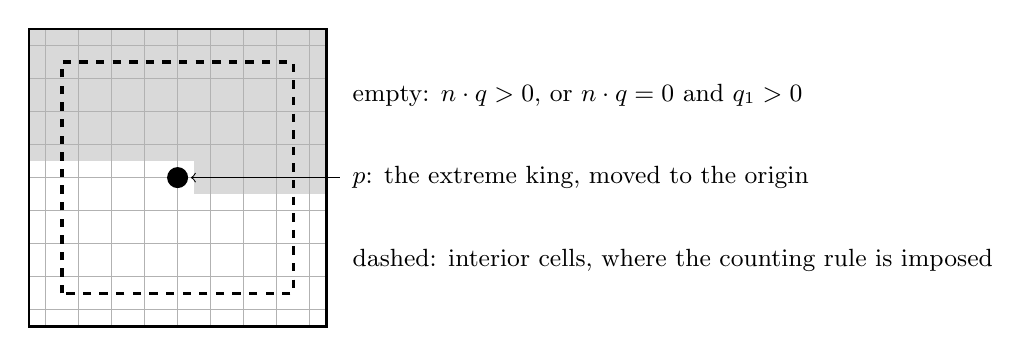
\begin{tikzpicture}[scale=0.42]
% cells [-4,4]^2, cell (x,y) drawn as the unit square centred at (x,y)
\foreach \x in {-4,...,4} \foreach \y in {1,...,4} \fill[black!15] (\x-0.5,\y-0.5) rectangle (\x+0.5,\y+0.5);
\foreach \x in {1,...,4} \fill[black!15] (\x-0.5,-0.5) rectangle (\x+0.5,0.5);
\draw[black!30] (-4.5,-4.5) grid (4.5,4.5);
\draw[thick] (-4.5,-4.5) rectangle (4.5,4.5);
\draw[very thick,dashed] (-3.5,-3.5) rectangle (3.5,3.5);
\filldraw[fill=black] (0,0) circle (0.3);
\node[right,font=\small] at (5,2.5) {empty: $n\cdot q>0$, or $n\cdot q=0$ and $q_1>0$};
\node[right,font=\small] at (5,0) {$p$: the extreme king, moved to the origin};
\node[right,font=\small] at (5,-2.5) {dashed: interior cells, where the counting rule is imposed};
\draw[->] (4.9,0) -- (0.4,0);
\end{tikzpicture}
